% VUT FIT MITAI
% MSZ 2021/2022
% Author: Vladimir Dusek
% Login: xdusek27

%%%%%%%%%%%%%%%%%%%%%%%%%%%%%%%%%%%%%%%%%%%%%%%%%%%%%%%%%%%%%%%%%%%%%%%%%%%%%%%%

\chapter{Hašovací funkce, klíčovaný haš a MAC a jejich použití a vlastnosti.}

%%%%%%%%%%%%%%%%%%%%%%%%%%%%%%%%%%%%%%%%%%%%%%%%%%%%%%%%%%%%%%%%%%%%%%%%%%%%%%%%

\section{Metadata}

\begin{itemize}
    \item Předmět: Kryptografie (KRY)
    \item Přednáška:
    \begin{itemize}
        \item \path{KRY04_Asym_MNG.pdf}
    \end{itemize}
    \item Záznam:
    \begin{itemize}
        \item 2021-03-22
    \end{itemize}
\end{itemize}

%%%%%%%%%%%%%%%%%%%%%%%%%%%%%%%%%%%%%%%%%%%%%%%%%%%%%%%%%%%%%%%%%%%%%%%%%%%%%%%%

\section{Úvod a kontext}

\textit{Viz. \uv{Úvod a kontext} v předchozích otázkách z tohoto předmětu.}

\paragraph*{Hashovací funkce} Hashovací funkce je funkce (resp. algoritmus) pro převod vstupních dat do (relativně) malého čísla. Výstup hashovací funkce se označuje otisk, \textit{fingerprint}, \textit{digest} či \textit{hash}. Jsou jednosměrné a odolné proti kolizím (viz vlastnosti).

\paragraph*{Obecné vlastnosti} Hashovací funkce by měla: \begin{itemize}
    \item Být aplikovatelná na argument o libovolné velikosti.
    \item Mít výstyp konstantní délky.
    \item Dokázat spočítat výstup rychle.
\end{itemize}

\paragraph*{Neklíčované hashovací funkce} Hashovací funkce má pouze jeden argument~--~data. Např. MD2, MD4, MD5, SHS, SHA1, SHA2, SHA3. $$f(data) \rightarrow hash$$

\paragraph*{Klíčované hashovací funkce} Hashovací funkce má dva argumenty~--~data a klíč. Také se jim někdy říká MAC (\textit{message authentication code}). $$f(data, key) \rightarrow hash$$

%%%%%%%%%%%%%%%%%%%%%%%%%%%%%%%%%%%%%%%%%%%%%%%%%%%%%%%%%%%%%%%%%%%%%%%%%%%%%%%%

\section{Kryptografická odolnost hashovacích funkcí}

\paragraph*{Vlastnosti z hlediska odolnosti} Hashovací funkce by z hlediska kryptografické odolnosti měly splňovat: \begin{itemize}
    \item \textit{First preimage resistance}~--~Pro konkrétní $y$ je výpočetně nezvládnutelné najít takové $x$, aby platilo $h(x) = y$. Útočník má k dispozici konkrétní hash, a snaží se pro něho nalézt zprávu.
    \item \textit{Second preimage resistance}~--~Pro konkrétní $x$ je výpočetně nezvládnutelné najít takové $x'$, aby platilo $h(x) = h(x')$. Útočník má k dispozici konkrétní zprávu (nemůže si ji zvolit), ke které se snaží nalézt jinou zprávu, která bude mít stejný hash.
    \item \textit{Collision resistance}~--~Je výpočetně nezvládnutelné najít libovolnou dvojici $x, x'$ takovou, aby platilo $x \neq x'$ a $h(x) = h(x')$. Útočník si může zvolit libovolnou zprávu, ke které se snaží nalézt jinou zprávu, která bude mít stejný hash. Pokud platí \textit{collision resistance}, tak platí i \textit{second preimage resistance}.
\end{itemize}

\paragraph*{Narozeninový problém} V teorii pravděpodobnosti je narozeninový problém úloha vypočítat minimální početnost skupiny lidí, ve které je alespoň 50\% pravděpodobnost nalezení dvojice se stejným datem narození. Narozeninovým paradoxem je pak označována skutečnost, že tento počet (23) je mnohem menší než intuitivní odhad.
Výsledek je intuitivnější, když uvážíme, že porovnání narozenin bude provedeno mezi všemi možnými dvojicemi jedinců. Při počtu 23 jedinců je třeba uvažovat $(23 \cdot 22) / 2 = 253$ dvojic, což je více než polovina počtu dnů v roce ($182,5$).

Jednodušší je nejprve spočítat jev opačný $\bar p(n)$, tedy pravděpodobnost, že všech $n$ narozenin je rozdílných. Pro $n > 365$ je $1$, jinak:
\begin{equation}
\begin{aligned}
\bar p(n) &= 1 \cdot \left(1-\frac{1}{365}\right) \cdot \left(1-\frac{2}{365}\right) \cdots \left(1-\frac{n-1}{365}\right) = \\
&=  \frac{365 \cdot 364 \cdots (365-n+1)}{365^n} = \\
&=  \frac{365!}{365^n (365-n)!}
\end{aligned}
\end{equation}

\begin{equation}
    p(n) = 1 - \bar p(n)
\end{equation}

\paragraph*{Narozeninový útok} Mějme hashovací funkci, která má $n$ bitový výstup (celkový počet možných hashů je $2^{n}$). Útočník vytvoří dokument \uv{přátelská dohoda} a přibližně $2^{n/2}$ sémanticky ekvivalentních verzí (úprava bílých znaků, úprava pořadí celků, jiné formulace, \dots). Podobně vytvoří dokument \uv{nepřátelská dohoda} a přibližně $2^{n/2}$ sémanticky ekvivalentních verzí. S pravděpodobností $0,5$ existuje verze \uv{přátelské dohody} a \uv{nepřátelské dohody}, které mají stejný hash. Pokud takové verze existují, útočník dá oběti podepsat \uv{přátelskou dohodu} $\Rightarrow$ existuje validní podpis \uv{nepřátelské dohody}.

\paragraph*{Bezpečnostní cíle OWHF} Bezpečnostní cíle OWHF (\textit{one way hash function}). Některé protokoly nevyžadují bezkoliznost, proto má smysl řešit i tento případ. \begin{itemize}
    \item Vyžadované vlastnosti: \textit{first preimage resistance} a \textit{second preimage resistance}
    \item Cíl útočníka: vytvořit \textit{first preimage} nebo \textit{second preimage} (oba úkoly jsou stejně těžké)
    \item Složitost: $O(2^n)$ ($n$ je počet bitů hashe)
    \item Požadovaná délka: $n \geq 80$
\end{itemize}

\paragraph*{Bezpečnostní cíle CRHF} Bezpečnostní cíle CRHF (\textit{collision resistance hash function}). \begin{itemize}
    \item Vyžadované vlastnosti: \textit{collision resistance}
    \item Cíl útočníka: vytvořit kolizi
    \item Složitost: $O(2^{n / 2})$ ($n$ je počet bitů hashe) (kvůli narozeninovému útoku)
    \item Požadovaná délka: $n \geq 160$
\end{itemize}

\paragraph*{Bezpečnostní cíle MAC} Bezpečnostní cíle MAC (\textit{message authentication code}). \begin{itemize}
    \item Vyžadované vlastnosti: \textit{computation resistance}, \textit{key non-recovery}
    \item Cíl útočníka (útočník si může vybrat): \begin{itemize}
        \item Vytvořit nový hash, který bude odpovídat nové zprávě
        \item Nalézt klíč
    \end{itemize}
    \item Složitost ($n$ je počet bitů hashe, $t$ je počet bitů klíče): \begin{itemize}
        \item Vytvořit nový hash: $O(max(2^{-n}, 2^{-t}))$
        \item Nalézt klíč: $O(2^n)$
    \end{itemize}
    \item Požadovaná délka: $n \geq 64 \; \land \; t \geq 64$
\end{itemize}

%%%%%%%%%%%%%%%%%%%%%%%%%%%%%%%%%%%%%%%%%%%%%%%%%%%%%%%%%%%%%%%%%%%%%%%%%%%%%%%%

\section{Hashovací funkce neklíčované}

Nejčastější způsoby sestrojení hashovací funkce neklíčované jsou založené na principu iterace.

\begin{figure}[H]
    \centering
    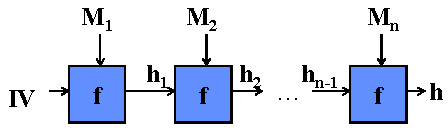
\includegraphics[width=0.6\linewidth]{kry_3/hash_function_iterative.pdf}
    \caption{Schéma iterativní neklíčované hashovací funkce. Zpráva je rozdělena na $n$ částí. $f$ je tzv. kompresní funkce. $IV$ je inicializační vektor, resp. konstanta. $h_1$ až $h_{n-1}$ jsou mezivýsledky (\uv{mezihashe}) a $h$ je výsledný hash.}
\end{figure}

\begin{figure}[H]
    \centering
    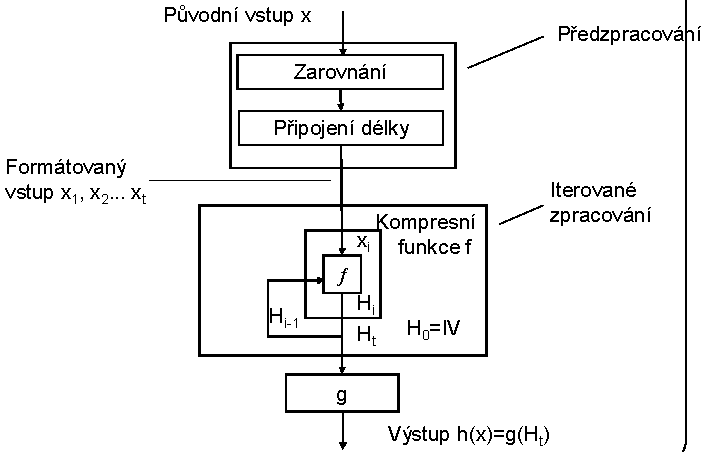
\includegraphics[width=0.9\linewidth]{kry_3/hash_function_iterative_detail.pdf}
    \caption{Podrobnější schéma iterativní neklíčované hashovací funkce.}
\end{figure}

Jednotlivé kroky hashovací funkce: \begin{itemize}
    \item Předzpracování~--~Vstupní data jsou rozdělena na bloky o stejné délce. Je provedeno zarovnání posledního bloku. Je připojena informace o délce zprávy.
    \item Iterativní zpracování~--~V iteracích se postupně \uv{přihashovávají} vstupní bloky. Zpět\-ná vazba pomocí stavové proměnné. Uvnitř kompresní funkce, která z delšího vstupu uděla kratší výstup.
    \item Postzpracování~--~Volitelný krok.
\end{itemize}

\paragraph*{Merkelova meta-metoda} Nechť $f$ je kompresní funkce odolná proti kolizím. Hashovací funkce $h$ na principu iterace využívající kompresní funkci $f$ je rovněž odolná proti kolizím.

\paragraph*{Merkel-Damgardovo zesílení} Pokud je do vstupu hashovací funkce vložena délka zprá\-vy, tak je zajištěno, že žádná zpráva není prefixem jiné zprávy.

\paragraph*{Zarovnání} Nejednoznačné zarovnání (\textit{ambiguous padding}) -- připoj ke zprávě tolik bitů, aby délka zprávy byla násobkem délky bloku. Jednoznačné zarovnání (\textit{unambiguous padding}) -- připoj ke zprávě jeden bit a poté proveď nejednoznačné zarovnání.

\subsection*{Hashovací funkce s využitím blokových šifer}

Alternativně lze využít pro konstrukci hashovacích funkcí blokové šifry. Avšak blokové šifry byly navrhovány pro jiný režim činnosti, kterém útočník nezná klíč (a není schopen ho ovlivnit), zná pouze šifrovaný text (ten je schopen ovlivnit). V tomto případě útočník může přimo ovlivňovat hodnoty klíče.

\begin{figure}[H]
    \centering
    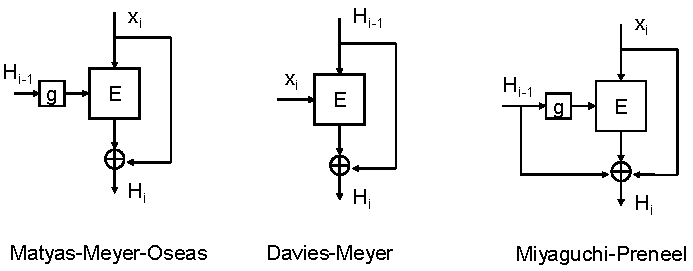
\includegraphics[width=0.9\linewidth]{kry_3/hash_function_blocks.pdf}
    \caption{Ukázka několika možných způsobů využití blokových šifer pro konstrukci kompresní funkce. S využitím iteračního způsobu lze zobecnit pro celou hashovací funkci.}
\end{figure}

%%%%%%%%%%%%%%%%%%%%%%%%%%%%%%%%%%%%%%%%%%%%%%%%%%%%%%%%%%%%%%%%%%%%%%%%%%%%%%%%

\section{MAC (\textit{message authentication code})}

\begin{itemize}
    \item Rodina hashovacích funkcí $h_k$, které jsou parametrizovatelné klíčem $k$.
    \item Vlasnosti (stejné jako u obecných hashovacích funkcí, pouze rozšířené o klíč): \begin{itemize}
        \item Výstup $h_k(x)$ lze spočítat rychle, pokud je znám klíč $k$.
        \item Jsou výpočetně bezpečné -- při znalosti dvojice $(x, h_k(x))$ je výpočetně nemožné spočíst novou dvojici $(x', h_k(x'))$, pro $x \neq x'$, pokud není znám klíč.
    \end{itemize}
    \item Využití: zajištění autentizace a integrity (nepopiratelnost zajistit nedokáže).
\end{itemize}

\begin{figure}[H]
    \centering
    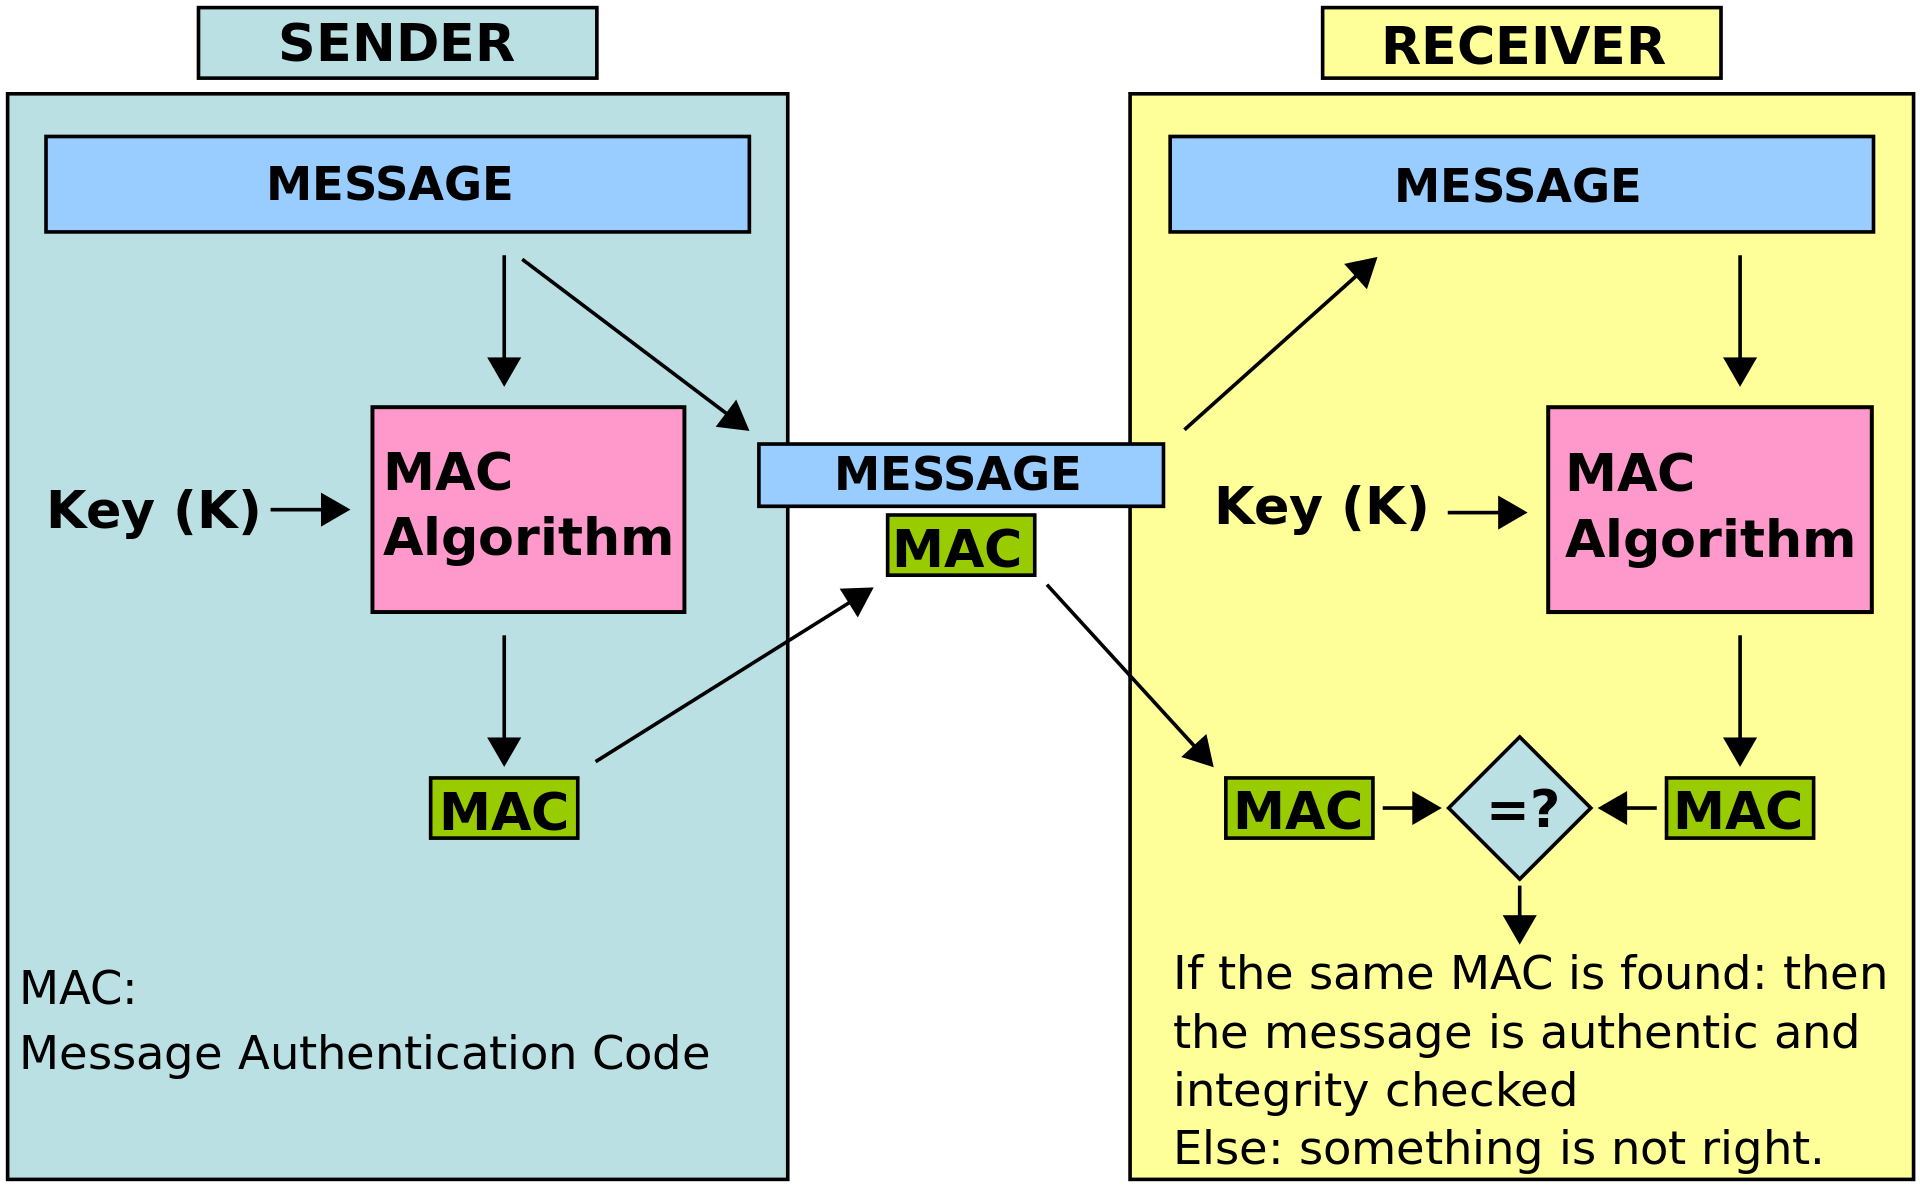
\includegraphics[width=1\linewidth]{kry_3/mac.png}
    \caption{Schéma použití MAC. Pokud je stejný MAC výpočítán na straně příjemce, tak má jistotu, že zpráva nebyla po cestě změněna a že zprávu poslal skutečně odesílatel.}
\end{figure}

\subsection*{Sestrojení MAC pomocí blokové šifry v CBC}

Pro sestrojení MAC hashovací funkce je využita symetrická bloková šifra v režimu CBC (\textit{cipher block chaining}, šifrová zpětná vazba). Rozdíl oproti CBC šifrování spočívá v tom, že mezivýsledky se zahazují a pracuje se až s posledním blokem. Z něho se vezme určitý počet posledních bitů (podle požadované délky hashe -- 32, 48, 64) a ten tvoří výsledný hash (MAC).

\begin{figure}[H]
    \centering
    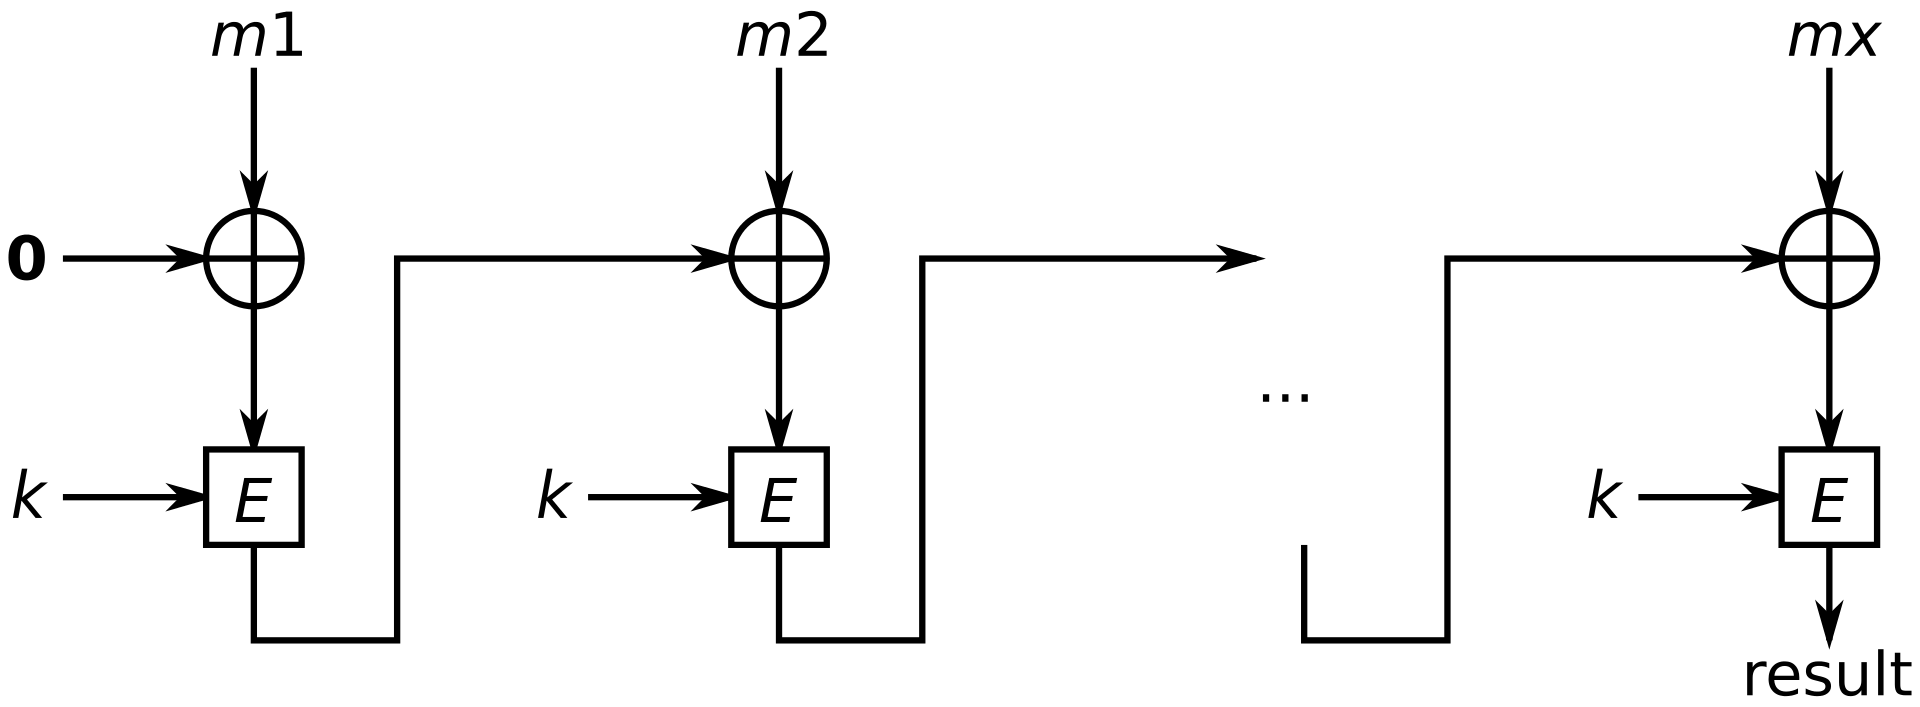
\includegraphics[width=0.8\linewidth]{kry_3/mac_cbc.png}
    \caption{Ukázka sestrojení MAC funkce pomocí symetrické blokové šifry v režimu CBC.}
\end{figure}

Proč stačí výrazně menší délka? Protože klíč. Útočník sice může vyzkoušet všechny možné hashe, ale bez znalostí klíče, nezjistí, který je ten správný.

\subsection*{Sestrojení MAC pomocí neklíčované hashovací funkce}

Pro sestrojení MAC hashovací funkce je využita neklíčovaná hashovací funkce. Klíč je připojen ke zprávě a je použita standardní hashovací funkce.

\paragraph*{Secret prefix} Klíč je přidán na začátek zprávy. Formálně: $H = h(k || x)$, kde $H$ je výsledný hash (MAC), $h$ je hashovací funkce, $k$ je klíč a $x$ je zpráva. Útočník může libovolně \uv{přihashovávat} další bloky bez znalosti klíče a tím vytvářet nové validní hashe~--~$h(k || x || y)$, kde $y$ je útočníkova zpráva $\Rightarrow$ nepřijatelný způsob.

\paragraph*{Secret suffix} Klíč je přidán na konec zprávy. Formálně: $H = h(x || k)$. Útočník, který může zvolit $x$, může také vytvořit $x'$, pro které $h(x) = h(x')$ se složitostí $O(2^{n/2})$, kde $n$ je délka hashe, bez ohledu na délku klíče $k$ (narozeninový útok) $\Rightarrow$ nepřijatelný způsob (útok který je neovlivnitelný délkou klíče).

\paragraph*{Enveloping} Klíč je přidán na začátek i na konec zprávy. Formálně: $H = h(k || p || x || k)$, kde $p$ je zarovnání. Přijatelný způsob. Základ pro algoritmus HMAC.

\subsection{HMAC (\textit{hash function MAC})}

HMAC (\textit{hash function MAC}) je do dnes používaný algoritmus. Specifikuje použití metody \textit{enveloping}, ale ne, která hashovací funkce se použije.

\begin{figure}[H]
    \centering
    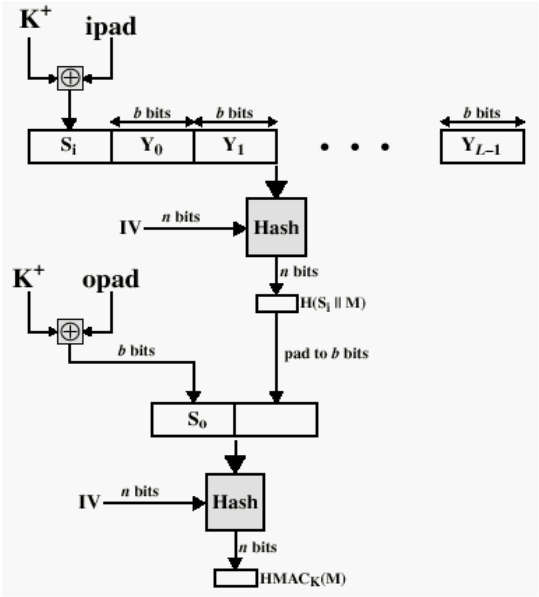
\includegraphics[width=0.9\linewidth]{kry_3/hmac.png}
    \caption{Schéma HMAC; \texttt{ipad} a \texttt{opad} jsou vstupní/výstupní konstanty, které slouží k zarovnání; $Y_i$ jsou bloky vstupní zprávy; $IV$ je inicializační vektor.}
\end{figure}
